Localizing and classifying activities in long untrimmed video is of great importance in video understanding ranging from video indexing to surveillance and robotics. Action segmentation is a video understanding task about identifying when and what type of action in a given video. This is done by temporally locating action segments in the video and classifying the action category of each segment. To capture long-range dependencies of action events in long untrimmed videos, recent methods using dilated temporal convolutions \cite{8953830,9186840} and dilated temporal graphs for temporal reasoning \cite{graphbased2020,wang2020temporal} have been very successful. While they can achieve decent performance on less complex datasets \cite{Ishikawa_2021_WACV}, the performance significantly drops when the models are evaluated on large, challenging datasets as indicated by \newcite{graphbased2020}. We see there is still room for performance improvement due to the inherent complexity of the task and the dataset.


\begin{figure}[t]
    \centering
    \begin{tikzpicture}[scale=0.7]
        \node[] at (4,-8) {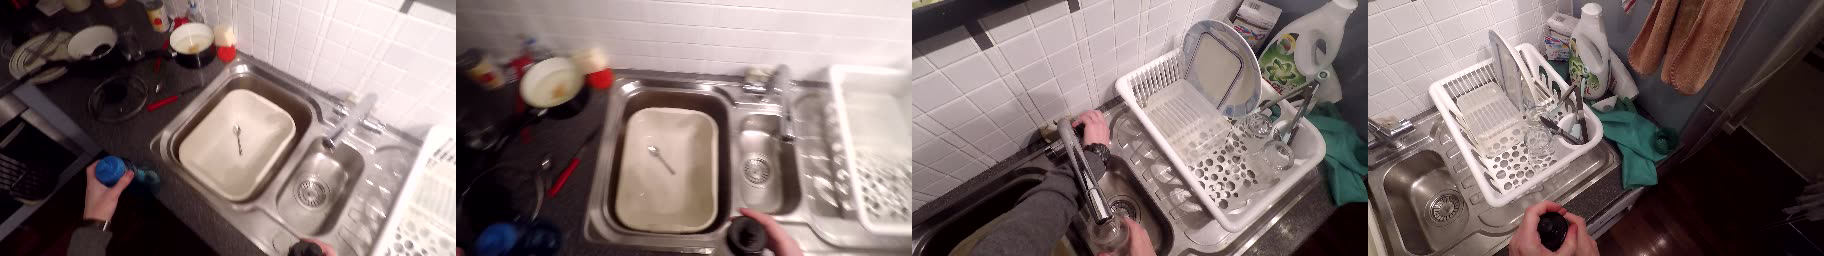
\includegraphics[scale=0.1]{figures/input.png}};
        \draw[->,-stealth,semithick] (4,-7.6) to (4,-6.5);
        
        \filldraw[fill=black!5!white,rounded corners=5] (2,-6.5) rectangle (6,-5.5) node[pos=0.5] {\small SS-TCN Stage 1};
        \draw[->,-stealth,densely dashed,semithick] (4,-5.5) to (4,-4.5);
        \filldraw[fill=black!5!white,rounded corners=5] (2,-4.5) rectangle (6,-3.5) node[pos=0.5] {\small SS-TCN Stage 4};
        \draw[rounded corners=5,densely dashed] (0,-7) rectangle (8,-3);
        \node[] at (7,-5) {\textbf{\textsf{\scriptsize Backbone}}};
        \draw[->,-stealth,semithick] (4,-3.5) to (4,-2.4);
        \filldraw[fill=red!40!white, draw=black] (0,-2.4) rectangle (2.5,-2);
        \filldraw[fill=cyan!40!white, draw=black] (2.5,-2.4) rectangle (6.5,-2);
        \filldraw[fill=blue!40!white, draw=black] (6.5,-2.4) rectangle (8,-2);
        \draw[] (0,-2.4) rectangle (8,-2) node[pos=0.5] {\small Prediction};

        \filldraw[fill=red!40!white, draw=black] (0,4) rectangle (2.5,4.4);
        \filldraw[fill=yellow!40!white, draw=black] (2.5,4) rectangle (6.5,4.4);
        \filldraw[fill=green!40!white, draw=black] (6.5,4) rectangle (8,4.4);
        \draw[] (0,4) rectangle (8,4.4) node[pos=0.5] {\small Prediction};
        \draw[->,-stealth,semithick] (4,-2) to (4,4);
        \filldraw[fill=black!5!white,rounded corners=5] (-0.5,0) rectangle (2.5,2) node[text width=2cm,pos=0.5,align=center] {\small Video-to-Text Retrieval};
        \filldraw[fill=black!20!white, draw=black] (-1.6,-1) rectangle (0.4,-0.5) node[pos=0.5] {\footnotesize Narrations};
        \draw[->,-stealth,semithick] (0.4,-0.75) -- (0.8,-0.75) -- (0.8,0);
        \draw[->,-stealth,semithick] (4,-0.75) -- (1.2,-0.75) -- (1.2,0);
        \draw[->,-stealth,semithick] (1,2) -- (1,2.5) -- (4,2.5);
        \draw[rounded corners=5,densely dashed] (-1.7,-1.5) rectangle (8,3.5);
        \node[text width=2.5cm, align=center] at (6,1) {\textbf{\textsf{\scriptsize Video-Text Retrieval Module}}};
    \end{tikzpicture}
    \caption{Overview of the proposed approach. The backbone model is MS-TCN, which is a stack of four single-stage TCNs (SS-TCN). Our video-text retrieval module extracts segments from the initial segmentation predicted by the backbone and retrieves the most relevant narration of each segment. Then the frame-wise classification label are updated with the verb in the retrieved narration.}
    \label{fig:overview-of-appraoch}
\end{figure}

There are two sub-challenges in action segementation, namely 1) localizing the events for action segments and 2) classifying the action in each segment. While the two sub-challenges are highly dependent on each other, we empirically found that misclassification is a more prominent issue. With the emerging field of multimodal machine learning, we are curious about whether additional information from textual modality will help mitigate the issue. Therefore, we propose a new architecture that combines temporal convolution networks with a video-to-text retrieval component. In contrast to previous works, our approach utilizes the semantic meaning of narrations to improve classification of localized action segments. We also experiment with textual inputs of different levels of complexity to see its impact on the performance. To the best of our knowledge, there is no prior work attempting at multimodal methods in solving the action segmentation task. The visual inputs are video frames extracted at a fixed frame rate, and the textual inputs are narrations describing action events in videos. We evaluate our model on the largest, egocentric cooking video dataset. A second contribution is that we experiment with textual inputs of various complexity levels and investigate their impact on the performance. This work is meaningful as it opens up a new research direction of multimodal action segmentation.
% Our contribution is two-folded:
% \begin{itemize}
%     \item Our proposed approach is the first attempt to action segmentation using multimodal inputs. The visual inputs are video frames extracted at a fixed frame rate, and the textual inputs are narrations describing action events in videos. We evaluate our model on the largest, egocentric cooking video dataset.
%     \item We experiment with textual inputs of various complexity levels and investigate their impact on the performance. This work is meaningful as it opens up a new research direction of multimodal action segmentation.
% \end{itemize}

